\chapter{Compressing Signatures}
\label{sec:compress}

Our second contribution, also in the form of an addition to the \sidh signature extension, is a mechanism for compressing signatures. The following chapter will cover the compression technique used. This chapter, much like the last, will be split into three sections: a brief coverage of the employed compression technique, the details of our implementation and integration of this technique into \sidh, and finally an analysis of the results of this contribution.

In the first section of this chapter, we discuss the SIDH public key compression technique resulting from combined efforts of Azerderakhsh et al. \cite{compwr} and Costello et al. \cite{pkcomp}. We attempt to provide a sufficient overview of the technique while only covering in detail the components that are of significant relevance to our implementation. Those who seek to better understand the ins and outs of this technique should direct themselves to the original papers.  

The second section covers in detail how we apply this public key compression to Yoo et al. signatures. We make use of the functions offered by Costello et al. which implement the previously mentioned technique. This code was first made available in the second installment of Microsoft's SIDH library \cite{sidhcode}.

Finally, we round off the Chapter with an analysis of the memory improvement offered by this technique. We contrast this spatial improvement with the computational cost of compressing points, and discuss the practicality of employing this technique. 

\section{SIDH Key Compression Background}

In this section we will breifly cover the literature surrounding the compression technique that we employ. This technique was first outlined by Azerderakhsh et al. \cite{compwr} and later improved upon by Costello et al. \cite{pkcomp}. Here we investigate the details of these works that are relevant to our implementation.\\

\noindent
First, recall from Section \ref{subsec:sidhkex} the structure of an SIDH public key, denoted $pk$;
$$
pk = (E, P, Q)
$$
Where $E$ is a supersingular elliptic curve and $P$ and $Q$ are elliptic curve points such that $P, Q \in E$. Recall that E can be sufficiently represented by one $\mathbb{F}_{p}$ element which denotes $A$ from the following definition of $E$:
$$
E : y^2 = x^3 + Ax + B,
$$

$A$ sufficiently represents $E$ in this context because in \sidh we are concerned only with curves where $B$ = 0. 

$P$ and $Q$, on the other hand, can each be represented by their $x$-coordinate (two $\mathbb{F}_{p}$ elements) and a single bit determining the correct $y$-coordinate. Therefore, without more sophisticated compression, an \sidh public key can be represented with $~6\log p$ bits.

\subsection{Compressing SIDH Public Keys}
\label{subsec:azercompression}

Recall the discrete logarithm problem in the context of elliptic curves: given an elliptic curve group $E(K)$ and points $P, Q \in E(K)$, find $n$ such that $P = nQ$. The two-dimensional discrete log problem is then the following: given an elliptic curve group $E(K)$, two points $\{R_1, R_2\}$ generating a subgroup $S$ of $E(K)$, and an element $s \in S$, compute $\alpha$ and $\beta$ such that:
$$
s = \alpha R_1 + \beta R_2
$$
The Pohlig-Hellman algorithm can be applied to solve the discrete logarithm problem in groups whose order is a smooth integer \cite{ph}, and there is a variation of this algorithm which solves this two-dimensional discrete log problem with time complexity $O(\sqrt[q]\log p)$, where $q$ is the largest prime dividing $\vert S\vert$ \cite{genph}.\\

\noindent
Azerderakhsh et al. show that an SIDH public key can be further compressed in the following way. Taking \alice's SIDH key pair, for example, we have her public key $\pka = (E_{\ba}, \pa(\genpb),\pa(\genqb))$ and her private key $\ska = \{\ma, \na\}$ such that $ker(\pa) = \langle [\ma]\genpa, [\na]\genqa\rangle$. Because $\{\genpb, \genqb\}$ generates the torsion subgroup $E_{\ba}[\lbeb]$, we have that $\pa(\genpb) \in E[\lbeb]$ and $\pa(\genqb) \in E[\lbeb]$. Thus, the Pohlig-Hellman algorithm can be used to resolve $\pa(\genpb) = \alpha_P R_1 + \beta_P R_2$ and $\pa(\genqb) = \alpha_Q R_1 + \beta_Q R_2$ where $\{R_1, R_2\}$ is a basis for $E_{\ba}[\lbeb]$ \cite{compwr}.

Then, instead of sending \bob $(E_{\ba}, \pa(\genpb),\pa(\genqb))$, \alice can send $(E_{\ba}, \alpha_P, \beta_P, \alpha_Q, \beta_Q)$.\footnote{The approach outlined by Azerderakhsh et al. involves sending the $j$-invariant of $E$, which can be represented with the same amount of space as one $\mathbb{F}_{p^2}$ element. Because we are working in \sidh where we can already represent curves with one $\mathbb{F}_{p^2}$ element, we ommit this detail.} And so, as long as \alice and \bob can seperately generate the same $\{R_1, R_2\}$, they can both sufficiently represent one anothers public keys with only $4\log p$ bits.\\

\noindent
\textit{Constructing the Basis}. Constructing $R_1$ and $R_2$ can be done with a relatively simple yet time consuming process. We will continue to use the compression of \alice's public key, $\pka$, as our example.
\begin{enumerate}
\item Choose a random point $P \leftarrow_{\$} E(\mathbb{F}_{p^2})$.
\item Multiply $P$ by $\lbeb \cdot f$ to obtain $P'$, the order of which will divide $\lbeb$.
\item Check the order of $P'$ by multiplying it by powers of $\la$ until the identity is given.
\item If the order is $\lbeb$, set $R_1 = P'$, otherwise return to step one.
\item Repeat the same process for a new random point $Q$ until $Q'$ of order $\lbeb$ is found.
\item Check that $Q'$ is independent of $R_1$ by computing their Weil pairing: $e(R_1, Q')$.
\item If the pairing results in anything other than 1, set $R_2 = Q'$, otherwise return to step 5.
\end{enumerate}
The same $(R_1, R_2)$ pair will be derived by both \alice and \bob if and only if they use a psuedorandom number generator for generating $P$ and $Q$ AND they run their PRNGs with identical seeds \cite{pwcomp}.\\

\noindent
\textit{Decompressing Public Keys}. Decompression for this technique varies depending on the setting, but for our purpose we are concerned only with how decompression is done for SIDH key exchange. \bob computes the basis $\{R_1, R_2\}$ by seeding his PRNG with the same value as \alice. \bob then uses $\alpha_P, \beta_P, \alpha_Q$ and $\beta_Q$ to recompute $\pa(\genpb)$ and $\pa(\genqb)$. Then \bob computes the isogeny $\phi'_{\rb} : E_{\ba} \rightarrow E_{\ba\rb}$ with $ker(\phi'_{B}) =$ \cite{compwr}. 

\alice then acts identically on \bob's now compressed public key, $\pkb$, and the two arrive at the same shared secret, the $j$-invariant of $E_{\ba\rb}$, just as in the original SIDH key exchange.\footnote{We have ommitted details from this method of compression that are concerned with potential \textit{twists} of \alice and \bob's curves when compressing public keys, as this does not play a role in our implementation. }

\subsection{Improvements to SIDH Key Compression}
\label{subsec:costcompression}

The work of Costello et al. further developed this approach to achieve public key sizes of $\frac{7}{2}\log p$ \cite{pkcomp}. In addition to this, Costello et al. also outline several algorithmic improvements which decrease the runtime of this compression mechanism.

Many of the algorithms offered by Costello et al. can be treated as black-boxes in our setting, and so finer grain details of their work on efficient compression are ommitted.\\

\noindent
\textit{Improved Compression.} Take \alice's public key $\pka$, compressed via the Azerderakhsh et al. technique, to be $(E_{\ba}, \alpha_{P}, \beta_{P}, \alpha_{Q}, \beta_{Q})$. Therefore we have
$$
P = \alpha_{P}R_1 + \beta_{P}R_2,
$$
$$
Q = \alpha_{Q}R_1 + \beta_{Q}R_2;
$$
Where $\{R_1, R_2\}$ forms a basis of $E_{\ba}[\laea]$, and $P$ and $Q$ are exactly the elliptic curve point components of \alice's original, uncompressed public key.

From here, Costello et al. note the following: The end goal of the key exchange (in our running example) is for \bob to compute $\langle P + \mb Q\rangle$, where $\mb$ is \bob's secretly generated value. Given that $P$ has order $n = \laea$, we have that either $\alpha_{P} \in \mathbb{Z}^{*}_{n}$ or $\beta_{P} \in \mathbb{Z}^{*}_{n}$, and so it follows that
$$
\langle P + \mb Q \rangle =  \begin{cases}
							\langle \alpha^{-1}_{P}P + \alpha^{-1}\mb Q \rangle & \text{if }\ \alpha_{P} \in \mathbb{Z}^{*}_{n}\\
							\langle \beta^{-1}_{P}P + \beta^{-1}\mb Q \rangle & \text{if }\ \beta_{P} \in \mathbb{Z}^{*}_{n}
							\end{cases}
$$
And so, computing $\langle P + \mb Q\rangle$ to arrive at the shared secret does not require recomputing $P$ and $Q$. Instead, the scalar factors of $P$ and $Q$ with respect to the generated basis can be normalized to yield
$$
(\alpha^{-1}_{P}P, \alpha^{-1}_{P}Q) = \begin{cases}
							(R_{1} + \alpha^{-1}_{P}\beta_{P} R_{2}, \alpha^{-1}_{P}\alpha_{Q}R_{1} + \alpha^{-1}_{P}\beta_{Q}R_{2}  & \text{if }\ \alpha_{P} \in \mathbb{Z}^{*}_{n}\\
							(R_{1} + \beta^{-1}_{P}\alpha_{P} R_{2}, \beta^{-1}_{P}\alpha_{Q}R_{1} + \beta^{-1}_{P}\beta_{Q}R_{2} & \text{if }\ \beta_{P} \in \mathbb{Z}^{*}_{n}
						   	\end{cases}
$$

And, thus, \alice has reduced the information she needs to send over the wire from $(E_{\ba}, \pa(\genpb), \pa(\genqb))$ to the following:
$$
\pka = \begin{cases}
	   (E_{\ba}, 0, \alpha^{-1}_{P}\beta_{P}, \alpha^{-1}_{P}\alpha_{Q}, \alpha^{-1}_{P}\beta_{Q}) & \text{if }\ \alpha_{P} \in \mathbb{Z}^{*}_{n}\\
	   (E_{\ba}, 1, \beta^{-1}_{P}\alpha_{P}, \beta^{-1}_{P}\alpha_{Q}, \beta^{-1}_{P}\beta_{Q}) & \text{if }\ \beta_{P} \in \mathbb{Z}^{*}_{n}
	   \end{cases}
$$
Or, alternatively we write
$$
\pka = \begin{cases}
	   (E_{\ba}, 0, \zeta_{P}, \alpha'_{Q}, \beta'_{Q}) & \text{if }\ \alpha_{P} \in \mathbb{Z}^{*}_{n}\\
	   (E_{\ba}, 1, \zeta'_{P}, \alpha'_{Q}, \beta'_{Q}) & \text{if}\ \beta_{P} \in \mathbb{Z}^{*}_{n}
	   \end{cases}
$$
For readability. This reduction from 4 $\mathbb{Z}^{*}_{n}$ elements to 3 takes \alice's compressed public key from $4\log p$ bits to $\frac{7}{2}\log p$ bits.\\

\noindent
\textit{Alternative Decompression.} Due to the loss of information in either $\alpha_{P}$ or $\beta_{P}$, an alternative route to secret agreement is required. For a compressed public key $(E, b, \zeta_{P}, \alpha_{Q}, \beta_{Q})$ there exists a $\gamma \in \mathbb{Z}^{*}_{n}$ such that
$$
(\gamma^{-1}P, \gamma^{-1}Q) = 
\begin{cases}
(R_1 + \zeta_{P}R_2, \alpha_{Q}R_1 + \beta_{Q}R_2) & \text{if }\ b = 0\\
(\zeta_{P}R_1 + R_2, \alpha_{Q}R_1 + \beta_{Q}R_2) & \text{if }\ b = 1
\end{cases}
$$
The verifier could reconstruct $\{R_1, R_2\}$ to produce $\langle P + mQ \rangle$ by computing $P$ and $Q$ from $\zeta_{P}, \alpha_{Q}, \beta_{Q}$ with $R_1$ and $R_2$, and then multiplying $Q$ by their private key $m$. This would require a 1-dimensional and a 2-dimensional scalar multiplication of points on the curve $E$. Costello et al. note instead that 
$$
\langle P + mQ \rangle = 
\begin{cases}
\langle (1 + m\alpha_{Q} R_1 + (\zeta_{P} + m\beta_{Q})R_2 \rangle & \text{if }\ b = 0\\
\langle (\zeta_{P} + m\alpha_{Q})R_1 + (1 + m\beta_{Q})R_2 \rangle & \text{if }\ b = 1
\end{cases}
$$
And since $n=l^{e}$ we have $(1 + m\alpha_{Q}), (1 + m\beta_{Q}) \in \mathbb{Z}^{*}_{n}$, giving
$$
\langle P + mQ \rangle = 
\begin{cases}
\langle R_1 + (1 + m\alpha_{Q})(\zeta_{P} + m\beta_{Q})R_2 \rangle & \text{if }\ b = 0\\
\langle (1 + m\beta_{Q})(\zeta_{P} + m\alpha_{Q})R_1 + R_2 \rangle & \text{if }\ b = 1
\end{cases}
$$
Reducing decompression to a single 1-dimensional scalar multiplication of a point on $E$ along with a handful of $\mathbb{F}_{p^{2}}$ operations.


\section{Implementation Details}
\label{sec:compimplementation}

In this subsection we demonstrate how the previously detailed public key compression technique can be used to compress Yoo et al.'s isogeny-based signatures. Again, we will turn to the \sidh library and reference portions of C code (some contributed by Patrick Longa \cite{sidhcode}, some by Yoo and his associates \cite{yoosigcode}, and some by us,) to investigate details of our implementations performance.\\

\noindent
Recall from \ref{sec:sigsbackground} the structure of a Yoo et al. signature, $\sigma$:
$$
\sigma = (com, ch, h, resp)
$$

\noindent
Where

\begin{itemize}
\item $com$ is a list of $2\lambda$ pairs of supersingular elliptic curves: $\{(E_{1,1}, E_{2,1}), (E_{1,2}, E_{2,2}), ..., (E_{1,2\lambda}, E_{2,2\lambda})\}$,
\item $ch$ is a list of $2\lambda$ randomly chosen bits,
\item $resp$ is a list of size $2\lambda$ where each element is either a single elliptic curve point $\pr(S)$, where $\pr$ is \randall's isogeny and $S$ is the signers secretly generated point, or the pair of points ($\cyr, \phi(\cyr)$), where \cyr is \randall's secretly generated point, and $\phi$ is the signers isogeny.
\item $h$ is a list of $2\lambda$ queries to a random oracle \textbf{G}, such that $h_{i} = \textbf{G(}resp_{i}\textbf{)}$
\end{itemize}

\noindent
Recall also from Subsection \ref{subsec:datarep} the following definitions:
\begin{itemize}
\item an \code{felm\_t} denotes a $\mathbb{F}_{p}$ element, e.g. a 751-bit element in \sidh,
\item an \code{f2elm\_t} denotes an $\mathbb{F}_{p^2}$ element, or two \code{felm\_t}s,
\item a \code{point\_affine} denotes an elliptic curve point represented in affine space (two \code{f2elm\_t}s), and
\item a \code{point\_proj} denotes an elliptic curve point represented in projective space (two \code{f2elm\_t}s).
\end{itemize}

\vspace{10px}
\noindent
The representation of $\sigma$ in \sidh (as implemented by Yoo et al.) has a few noteworthy differences. Signatures in this setting are defined via a C \code{struct} in the following way:\\

\begin{lstlisting}
struct Signature {
	f2elm_t *Commitments1[NUM_ROUNDS];
	f2elm_t *Commitments2[NUM_ROUNDS];
	unsigned char *HashResp;
	felm_t *Randoms[NUM_ROUNDS/2];
	point_proj *psiS[NUM_ROUNDS/2];
};
\end{lstlisting}
\vspace{15px}

With \code{NUM\_ROUNDS} equal to $2\lambda$. The bit-level security of a given signature, then, can be computed as $\code{NUM\_ROUNDS}/2$.

\code{Commitments1} is an array containing the first entry from every pair in $resp$, e.g.\ $\{E_{1,1}, E_{1,2}, ..., E_{1,2\lambda}\}$, and \code{Commitments2} holds the second entry from each pair. 

\code{HashResp} contains the elements of $h$. In practice the Keccak function\footnote{Keccak is a cryptographic hash function from which the newly standardized SHA-3 is based.} is used in place of the random oracle \textbf{G}. 32-byte hash digests are computed using Keccak such that \code{HashResp[i]} = \code{Randoms[i/2]} if the challenge bit $ch$ is 0, and \code{HashResp[i]} = \code{psiS[i/2]} if $ch$ is 1.

\code{Randoms} is an array of $\lambda$ \code{felm\_t}'s. The element at index $i$ of \code{Randoms} holds $\mr_{i}$, and represents \randall's secretly generated $\mathbb{F}_{p}$ value for iteration $i$ of the signing algorithm. These values sufficiently represent the elements of $resp$ which take the form ($\cyr, \phi(\cyr)$) for two reasons: 
\begin{enumerate}
\item $\cyr$ can be reconstructed using the torsion subgroup generating points that correspond to \randall ($\cyr = \genpa + \mr_{i}\genqa$ if \bob is signing, and $\cyr = \genpb + \mr_{i}\genqb$ if \alice is signing)
\item Because isogenies are (structure preserving) morphisms, it holds that $\cyr = P + [\mr]Q \Rightarrow \phi(\cyr) = \phi(P) + [\mr]\phi(Q)$. Thus, because $\phi(P)$ and $\phi(Q)$ are members of the signers public key, $\mr$ is sufficient for reconstructing $\phi(\cyr)$.
\end{enumerate}

Lastly, \code{psiS} denotes the elements of $resp$ which take the form of $\pr(S)$. These points cannot be represented by a single \code{felm\_t} (as in \code{Randoms}) because doing so would leak the signers private information.\\

\noindent
And so, the total size of an uncompressed \sidh signature, in bytes, is $
(\code{sizeof(felm\_t)} + \code{sizeof(f2elm\_t)} + \code{sizeof(f2elm\_t)} + \code{sizeof(point\_proj)} + 32) \cdot 2\lambda + (\code{sizeof(felm\_t)} + \code{sizeof(point\_proj)}) \cdot \lambda  = $.

\subsection{$\psi(S)$ Compression}

For the following subsection we will assume the signer to be \bob (e.g. using \rb values) and the verifier to be \alice (e.g. using \ba vaues). This is done only for simplicities sake - to reverse the roles one need only swap all \textcolor{blue}{blue} variables with their \textcolor{red}{red} counterparts, and vice-versa. Similarly, function names ending in \code{\_B} can be replaced with their \code{\_A} alternatives, and vice-versa.\\

\noindent
We employ the compression technique covered in the previous section to compress every element of \code{psiS} individually. This requires an additional bit value \code{compressed} in the \code{Signature} struct. It is important that this bit is packaged as part of the final signature so that the verifier knows whether or not they need to perform decompression. 

Recall that \bob has private key $\skb = \mb$ from which we can generate $S = \genpb + [\mb]\genqb$ and $\pb: E \rightarrow E/\langle S \rangle$, and public key $\pkb = (E_{\rb}, \pb(\genpa), \pb(\genqa))$. Recall also from previous sections that the general procedure for signature signing begins with \bob calling the \code{isogeny\_sign} function, which in turn spawns $2\lambda$ threads, each executing \code{sign\_thread}. Each of these threads has an identifier \code{r}, and performs the following via \code{sign\_thread}:
\begin{enumerate}
\item Makes a call to \code{KeyGeneration\_A} to generate \randall's keypair $(\pkr, \skr)$
\begin{itemize}
\item $\skr = \mr$
\item $\pkr = (E_{\cyr}, \pr(\genpb), \pr(\genqb))$ where $\pr: E \rightarrow E_{\cyr}$
\end{itemize}
\item Sets \code{Randoms[r]} $\gets \skr$
\item Sets \code{Commitments1[r]} $\gets E_{\cyr}$
\item Performs \code{SecretAgreement\_B} with $\skb$ and $\pkr$ to generate $(E_{\rb\cyr}, \pr(S))$.
\item Sets \code{Commitments2[r]} $\gets E_{\rb\cyr}$
\item Sets \code{psiS[r]} $\gets \pr(S)$
\end{enumerate}

And so, if we wish to apply point compression to \code{psiS}, we must invoke our compression function within every \code{sign\_thread} instance, after the execution of \code{SecretAgreement\_B}. 

\begin{figure}[!h]
\begin{lstlisting}
generate_3_torsion_basis(A_temp, P, Q, CurveIsogeny);
\end{lstlisting}
\caption{Generate a basis for $E[\lbeb]$}
\label{code:sigstruct}
\end{figure}

\begin{figure}[!h]
\begin{lstlisting}
for (int i=0; i < 238; i++) {
	xTPL(Pnot, Pnot, A_temp, CurveIsogeny->C);
	xTPL(Qnot, Qnot, A_temp, CurveIsogeny->C);

	if (is_felm_zero(((felm_t*)Pnot->Z)[0]) 
	 && is_felm_zero(((felm_t*)Pnot->Z)[1])) {
		return ERROR;
	}
	if (is_felm_zero(((felm_t*)Qnot->Z)[0]) 
	 && is_felm_zero(((felm_t*)Qnot->Z)[1])) {
		return ERROR;
	}
}
\end{lstlisting}
\caption{Checking the order of the newly constructed basis}
\label{code:checkorder}
\end{figure}

\begin{figure}[!h]
\begin{lstlisting}
Mont_ladder(R1->x, a, aR1, Pnot, A24, CurveIsogeny->oBbits, CurveIsogeny->owordbits, CurveIsogeny);
Mont_ladder(R2->x, b, bR2, Qnot, A24, CurveIsogeny->oBbits, CurveIsogeny->owordbits, CurveIsogeny);
\end{lstlisting}
\caption{Generate a basis for $E[\lbeb]$}
\label{code:sigstruct}
\end{figure}

\begin{figure}[!h]
\begin{center}
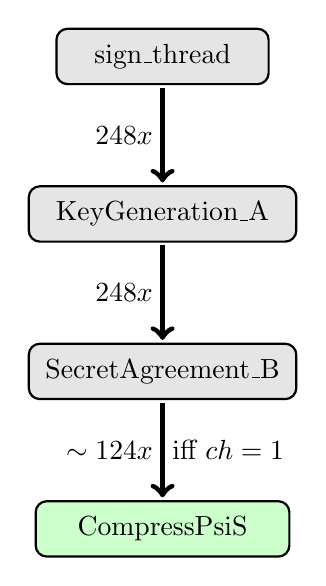
\begin{tikzpicture}
    [auto,
    block/.style={
      rectangle,
      draw=black,
      thick,
      fill=gray!20,
      text width=7em,
      align=center,
      rounded corners,
      minimum height=2em
    },
    block1/.style={
      rectangle,
      draw=black,
      thick,
      fill=gray!20,
      text width=9em,
      align=center,
      rounded corners,
      minimum height=2em
    },
	block2/.style={
      rectangle,
      draw=black,
      thick,
      fill=green!20,
      text width=8.5em,
      align=center,
      rounded corners,
      minimum height=2em
    },
    line/.style={
      draw,thick,
      -latex',
      shorten >=2pt
    },
    cloud/.style={
      draw=red,
      thick,
      ellipse,
      fill=red!20,
      minimum height=1em
    }
  ]
    \draw (1,-2) node[block] (A) {\code{sign\_thread}};
    \draw (1,-4) node[block1] (C) {\code{KeyGeneration\_A}};
	\draw (1,-6) node[block1] (D) {\code{SecretAgreement\_B}};
	\draw (1,-8) node[block2] (J) {\code{CompressPsiS}};
	\draw[->, line width=2.0] (1,-2.4) -- (1,-3.6) node[right] {};
		\draw (1, -3) node[left] (LABEL1) {$248x$};
	\draw[->, line width=2.0] (1,-4.4) -- (1,-5.6) node {};
		\draw (1, -5) node[left] (LABEL6) {$248x$};
	\draw[->, line width=2.0] (1,-6.4) -- (1,-7.6) node {};
		\draw (1, -7) node[left] (LABEL9) {$\sim124x$};
		\draw (1, -7) node[right] (LABEL10) {iff $ch = 1$};

\end{tikzpicture}
\end{center}
\caption{The general execution flow of \code{sign\_thread} with the addition of $\psi(S)$ compression}
\label{fig:signcallgraph}
\end{figure}

\subsection{Verifying A Compressed Signature}

If we look back to the SIDH public key decompression mechanism described in Subsection \ref{subsec:costcompression}, we note again that the aim is \textit{not} to reconstruct the originally compressed values ($\pa(\genpb)$ and $\pa(\genqb)$ in \alice's case.) Instead, an instance of compressed SIDH key exchange is able to arrive at the shared secret $j(E_{\ba\rb})$ between \alice and \bob without reconstructing the original points, by absorbing the constants into the shared secret value.

And so, the C code for the decompression procedure offered by Costello et al. cannot be directly applied in our setting, as it will not reconstruct the original $\psi{S}$ value. Moreover,

\begin{figure}[!h]
\begin{center}
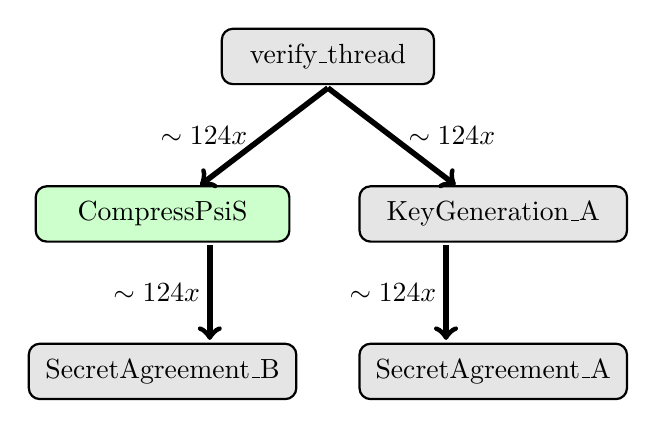
\begin{tikzpicture}
    [auto,
    block/.style={
      rectangle,
      draw=black,
      thick,
      fill=gray!20,
      text width=7em,
      align=center,
      rounded corners,
      minimum height=2em
    },
    block1/.style={
      rectangle,
      draw=black,
      thick,
      fill=gray!20,
      text width=9em,
      align=center,
      rounded corners,
      minimum height=2em
    },
	block2/.style={
      rectangle,
      draw=black,
      thick,
      fill=green!20,
      text width=8.5em,
      align=center,
      rounded corners,
      minimum height=2em
    },
    line/.style={
      draw,thick,
      -latex',
      shorten >=2pt
    },
    cloud/.style={
      draw=red,
      thick,
      ellipse,
      fill=red!20,
      minimum height=1em
    }
  ]
	\draw (9.5,-2) node[block] (B) {\code{verify\_thread}};
    \path (11.6,-4) node[block1] (E) {\code{KeyGeneration\_A}}
          (11.6,-6) node[block1] (F) {\code{SecretAgreement\_A}}
		  (7.4,-4) node[block2] (G) {\code{CompressPsiS}};
	\draw (7.4,-6) node[block1] (J) {\code{SecretAgreement\_B}};
	\draw[->, line width=2.0] (9.5,-2.4) to (E) node[above] {};
		\draw (8.6, -3) node[left] (LABEL4) {$\sim124x$};
	\draw[->, line width=2.0] (9.5,-2.4) to (G) node[right] {};
		\draw (10.4, -3) node[right] (LABEL5) {$\sim124x$};
	\draw[->, line width=2.0] (11,-4.4) -- (11,-5.6) node {};
		\draw (11, -5) node[left] (LABEL8) {$\sim124x$};
	\draw[->, line width=2.0] (8,-4.4) -- (8,-5.6) node {};
		\draw (8, -5) node[left] (LABEL9) {$\sim124x$};

\end{tikzpicture}
\end{center}
\caption{The general execution flow of \code{verify\_thread} with the addition of $\psi(S)$ compression}
\label{fig:verifycallgraph}
\end{figure}

\section{Results}

Looking at the storage requirements for the following. Figure \ref{table:spacereq} outlines the space requirements for different data structures in \sidh. From this information we can build up the data requirements based on  

Our technique can reduce the size of \sidh signature compression from \_\_\_ bits to \_\_\_ bits.\\

\noindent
\textit{Performance Measurements for Compressed Signatures}.

Because of how the signature extension of \sidh was originally written, our benchmarks reflect the time it takes for the signer to compress \code{psiS} for all $2\lambda$ iterations. In a finalized implementation of this system, significant time can be saved if the signer computes the challenge for an interation before compressing \code{psiS}, this will allow them to avoid running the compression procedure in cases where \code{psiS} is not part of the final signature, effectively reducing the time spent compressing points by a 50\%.

\subsection{Analysis}



\subsection{Potential Performance Improvements}

could use a non-constant implementation of double and add instead of montgomery's ladder? 

